\documentclass[11pt,a4paper]{article}
\usepackage[T1]{fontenc}
\usepackage[utf8]{inputenc}
\usepackage{lmodern}
\usepackage[margin=23mm,headheight=15pt]{geometry}
\usepackage{microtype,amsmath,amssymb,booktabs,longtable,tabularx,array}
\usepackage{graphicx,xcolor,enumitem,fancyhdr,placeins,xurl}
\usepackage{hyperref}
\definecolor{ink}{HTML}{183444}
\definecolor{accent}{HTML}{087F8C}
\definecolor{soft}{HTML}{EDF5F6}
\hypersetup{colorlinks=true,linkcolor=accent,urlcolor=accent,citecolor=accent,
 pdftitle={Video2Reaction: Experiments, Results, and Interpretation},
 pdfauthor={Video2Reaction research project}}
\pagestyle{fancy}
\fancyhf{}
\fancyhead[L]{\small\textcolor{ink}{Video2Reaction research report}}
\fancyhead[R]{\small 1 October 2026}
\fancyfoot[C]{\small\thepage}
\renewcommand{\headrulewidth}{0.3pt}
\setlength{\parindent}{0pt}
\setlength{\parskip}{5pt}
\setlength{\emergencystretch}{2em}
\setlist{itemsep=2pt,topsep=4pt,leftmargin=*}
\renewcommand{\arraystretch}{1.13}
\setcounter{tocdepth}{1}
\newcommand{\tbl}[1]{\input{tables/#1.tex}\FloatBarrier}
\newcommand{\KL}{\operatorname{KL}}
\newcommand{\softmax}{\operatorname{softmax}}
\newcommand{\LN}{\operatorname{LN}}
\newcommand{\GELU}{\operatorname{GELU}}
\newcommand{\code}[1]{\texttt{#1}}
\raggedbottom

\title{\textcolor{ink}{\textbf{Video2Reaction}}\\[5pt]
Experiments, Results, and Interpretation\\[5pt]
\large Controlled visual baselines and an audit of the research hypotheses}
\author{Research branch: \texttt{research/video2reaction-experiments}}
\date{1 October 2026\\\small Experiment results: 30 September 2026; cluster rechecked 00:38 UTC, 1 October}

\begin{document}
\maketitle
\begin{abstract}
This report describes the completed first experimental batch for predicting a distribution over 21 audience reactions from movie-clip keyframes. Five configurations were evaluated on the original Video2Reaction splits: a constant training-label prior (B0), frozen SigLIP2 features with mean pooling (B1), a temporal transformer (B2), its matched position-free set control, and a composite distribution/ranking objective (A5). All five runs and the shared 455,226-frame feature cache completed successfully on Snellius.

B1 reduces test KL from 0.689281 to 0.544414, a 21.0\% improvement over B0. Its paired movie-cluster bootstrap interval supports this gain. Differences in test KL between the learned models are inconclusive. B2 is sensitive to frame order, but does not clearly outperform its matched set control. A5 has small favorable cosine and ranking differences without evidence of a KL advantage. Weighted scores conceal weak rare-class performance, and 95.94\% of test clips share a movie with training. Peak selection, global-plus-peak fusion, VAD learning, and description diagnostics have not yet been run. Consequently, these results establish a viable visual baseline, but do not decide whether sparse emotional peaks, narrative context, or VAD geometry explain audience reactions.
\end{abstract}

\vspace{4pt}
\colorbox{soft}{\parbox{0.94\textwidth}{\textbf{Reading this report.} Sections 1--8 explain the evidence and its limits. Sections 9--10 distinguish untested hypotheses and give reproduction commands. Appendices contain the full class taxonomy, per-class metrics for every model, and 20 selected prediction examples. The report is understandable without the conversation or repository notes.}}
\clearpage
\tableofcontents
\clearpage

\section{Research question and scope}
Video2Reaction pairs clips with distributions of reactions inferred from viewer comments. The task concerns \emph{induced} audience reactions, which can differ from the emotion conveyed by a scene or expressed by its characters \cite{paper}. For clip $i$, the target $p_i\in\mathbb{R}^{21}$ is a nonnegative distribution with $\sum_c p_{ic}=1$. A predictor outputs $q_i$ in the same fixed class order.

The original research objective was to establish reproducible baselines, then test whether reaction prediction benefits from emotionally salient frames, reaction-specific attention, and global context. The first batch deliberately established reference points before these extensions. It evaluated visual-only prediction from frozen image representations. No audio, clip descriptions, genre, or movie identifier was supplied to these predictors. Movie IDs were used only for evaluation diagnostics and uncertainty grouping.

\subsection{What is established}
\begin{enumerate}
\item Frozen visual features and a small learned head improve substantially over a constant training-label prior on the official splits.
\item The simplest trained baseline, B1, has the lowest validation KL and the lowest point estimate of test KL among the evaluated models.
\item B2 trades better MRR, Top-1 F1, Chebyshev, intersection, and target-dominant probability error for worse KL and Top-3 F1 than B1. It has no clear test-KL advantage over its matched set control.
\item A5 slightly improves cosine, MRR, and Top-3 F1 over B1, while KL is almost unchanged. One fixed coefficient choice and one training seed do not establish objective superiority.
\item The infrastructure is verified: pinned splits and backbone, a locked uv environment, complete features, isolated source releases, resumable training, saved predictions, and a locked shared registry.
\end{enumerate}

\subsection{What is not established}
This batch cannot determine whether emotionally intense peaks are more useful than uniformly integrated frames, whether global context complements peaks, or whether VAD supervision helps. It also cannot rule out temporal models generally. Those claims require interventions that were not executed here. A failed attempt to start feature extraction was an infrastructure failure, not negative evidence about a model.

The project preserved the existing multimodal and VLM interfaces and added an isolated experiment package. This is a reproducible visual baseline study, not an exact reproduction of a published VLM or a claim to match its resource budget. The result provenance is the completed run artifacts and the committed aggregate JSON \cite{results,code}.

\section{Dataset and split audit}
\subsection{Inventory and available information}
The dataset was inspected on Snellius before code changes. The official metadata is pinned to revision \nolinkurl{578d1423f89f1a7b52471b01e78770e08f0a226c} of \nolinkurl{infofusionlab/Video2Reaction} \cite{dataset}. Original split membership is preserved.
\tbl{dataset}

All 10,348 official clips have a frame index and every referenced JPEG. No index has non-increasing start-frame numbers. The parent frame tree contains 1,390 additional clip directories; these are excluded. There are 455,226 referenced JPEGs and 10,348 CSV indices. The audit found no missing paths. Completed extraction subsequently decoded every referenced image.

Across all official clips, frame counts range from 15 to 176, with mean 43.9917 and median 39. Percentiles 1/5/25/50/75/95/99 are 15/15/25/39/58/89/115. The observed minimum is 15, while the paper lists 16 \cite{paper}. Image-size checks covered 207 systematically sampled first-frame headers: 197 were $640\times360$, nine were $534\times360$, and one was $536\times360$. This size survey was a sample, not an exhaustive resolution census.

Each \path{index.csv} records scene number, start/end time, and start/end frame. A zero-based scene number maps to a one-based filename such as \path{001.jpg}. Thus, chronological order and scene intervals are available. The experiments use ordered static keyframes; they do not observe all motion or audio between scenes.

All official targets are finite, nonnegative, and normalized within floating-point tolerance. Every clip has a description, IMDb ID, and movie name. Some lack genre: 1,594 training, 231 validation, and 452 test clips. The inspected split files provide one aggregated reaction distribution per clip, rather than individual comments or longitudinal reaction trajectories.

\subsection{Class order and imbalance}
The class order is fixed because CAD depends on cumulative sums along that order. Appendix~\ref{app:taxonomy} lists all 21 classes and their training mass. Admiration, disapproval, and amusement account for about 68.59\% of mean training target mass. The largest-to-smallest mean probability ratio is 174.17. This is a specific definition of imbalance and should not be equated with a differently defined published imbalance factor.

The targets often contain ties: 562 training, 81 validation, and 159 test clips have tied maximal probabilities. Metadata dominant labels lie among these maxima but can differ from a numerical argmax. Official top-k support therefore need not equal metadata dominant-label counts.

\subsection{Movie overlap and leakage limits}
No duplicate video IDs or exactly identical descriptions were found across splits. Content-level near-duplicate detection was not performed. Train/validation share 722 movie IDs; train/test share 1,110; validation/test share 568. Crucially, \textbf{1,986 of 2,070 test clips (95.94\%) come from movies present in training}; only 84 test clips are from unseen movies.

The official split remains the primary benchmark. It measures prediction on held-out clips under substantial movie overlap, not generalization to wholly new movies. Visual features can capture movie-specific appearance even without an explicit movie-ID input. Future movie-prior and same-movie-excluded comparisons would test this alternative explanation more directly.

\section{Implementation, environment, and execution checks}
\subsection{Repository changes and compatibility}
The original repository contained a multimodal temporal-convolution/context-attention model, CubeMLP training, classical label-distribution baselines, and VLM evaluation/LoRA entrypoints. It lacked a locked project environment, checked-in experiment configurations, SLURM jobs, and a common registry. The new work added \path{src/experiments/}, \path{train.py}, YAML configurations, and submission/collection helpers while retaining the old interfaces.

The audit identified an unassigned reaction-class constant and a missing, working-directory-dependent NRC lexicon path; these were corrected. Other legacy issues were documented: probability outputs being used as logits in a legacy loss, an in-memory best-checkpoint reference that could track later updates, and a standalone JS function with an extra sample-count division. The new path uses logits correctly, reloads serialized selected weights, and has its own mathematically correct JS training objective. Required official metric definitions were retained.

\subsection{Environment and shared feature cache}
Actual extraction, training, and model evaluation ran on Linux SLURM nodes using uv. The recorded environment is Python 3.11.16, PyTorch 2.8.0 with CUDA 12.8, Transformers 4.57.1, NumPy 2.2.6, scikit-learn 1.7.2, and Pillow 11.3.0. \path{pyproject.toml} and \path{uv.lock} define the environment. W\&B is optional. Local conda \code{torch} was used for synthetic checks and report preparation; the Mac did not run the benchmark models.

The common backbone is \nolinkurl{google/siglip2-so400m-patch14-384}, revision \nolinkurl{e8e487298228002f3d8a82e0cd5c8ea9c567f57f} \cite{siglip}. It is frozen and run in evaluation mode. Images are processed by the pinned image processor at its configured 384-pixel input resolution. Extraction uses bf16 computation and saves 1,152-dimensional float32 features. All indexed frames are retained, with image-byte hashes, frame provenance, split hashes, and feature/index checksums. Readers reject incomplete or incompatible caches. Extraction resumes from a flushed progress cursor.

The cache was built once on one A100 in 1h50m35s. The four learned predictors used MIG GPU slices and completed in 2m42s--2m43s each; these short runtimes exclude the shared backbone extraction. Comparing head runtime alone would understate total experimental cost.

\subsection{Three-video smoke tests}
Each GPU smoke uses the same three official \emph{training} clips: \code{4nSkJZ3i2-g}, \code{eiqBbLVXbQg}, and \code{iKp5ARBBpyc}. Eight chronological frames per clip give 24 frames in total. Mean pooling, the temporal transformer, composite loss, and reaction-query attention each run 25 optimization steps. Checks cover finite normalized predictions, decreasing training loss, exact checkpoint reload, and a resumed optimizer step.

\begin{table}[!htbp]\centering\small
\begin{tabular}{llll}\toprule
Smoke job & Source & Verification & Elapsed \\\midrule
27381153 & \code{08b8c30} & 14 tests + 3-video integration & 8m04s \\
27381915 & \code{e91a469} & 21 tests + 3-video integration & 5m41s \\
27382205 & \code{bbf8c1d} & 22 tests + shared-loader integration & 3m31s \\\bottomrule
\end{tabular}
\caption{All three smoke jobs completed with exit 0:0. These are environment and code checks. Their training-example losses are not benchmark results.}\label{tab:smoke}
\end{table}\FloatBarrier

The final smoke losses were 0.028483 for mean pooling, 0.012147 for the temporal model, 0.024368 for the composite objective, and 0.033656 for query attention. The objectives differ and the same three training examples are reused. These numbers must not be used to rank the research hypotheses.

\subsection{Failure, recovery, and run isolation}
The first full extraction job, 27382107, failed because \code{AutoProcessor(use\_fast=False)} selected an unused slow text tokenizer requiring SentencePiece. This was a mismatch between the smoke and production loaders. The fix uses a shared \code{AutoImageProcessor} loader in both paths. A cache round-trip regression and the third real GPU smoke passed before replacement submission.

The four dependent first-attempt jobs, 27382109--27382112, were cancelled before training. Their registry entries retain failed terminal status; their precise scheduler cause is dependency cancellation. Completed B0 job 27382108 was preserved. The corrected feature job 27382293 and learned jobs 27382294--27382297 then completed successfully. No failed infrastructure attempt is interpreted as a model result.

Jobs execute from verified frozen source directories, preventing subsequent code synchronization from changing queued experiments. The shared uv environment is not mutated by runs; execution uses \code{uv run --frozen --no-sync}. Checkpoints record model, optimizer, RNG, epoch, history, selected weights, and patience. Resume requires the same configuration and source identity. Synthetic interrupted/resumed training matches the uninterrupted trajectory; this does not promise bitwise equality across different GPU hardware.

The shared JSON registry uses an exclusive file lock and atomic writes. It rejects terminal-state regression and run-ID/job-ID conflicts. Per-run metrics remain the source of truth alongside scheduler state, so the global registry is not the only record. Submission locks and persisted job IDs prevent blind duplicates.

\section{Completed experiments and controlled comparisons}
\subsection{Common representation and training}
Let $x_{it}=f_\theta(I_{it})\in\mathbb{R}^{1152}$ be the frozen feature for frame $t$ of clip $i$. The shared learned projection is
\begin{equation}
u_{it}=W_P\LN(x_{it})+b_P\in\mathbb{R}^{128},\qquad
\operatorname{head}(h)=W_2\GELU(W_1h+b_1)+b_2.
\end{equation}
Thus, this B1 implementation applies per-frame layer normalization and a linear projection before averaging. It should be reproduced from this definition, rather than assumed to be a raw-feature mean followed by an arbitrary classifier. The output is $q_i=\softmax(z_i)$ over 21 classes.

All learned runs use seed 42, the same fixed splits and frozen cache, batch size 64, AdamW with learning rate $10^{-3}$ and weight decay $10^{-4}$, a constant learning rate, gradient clipping at 1.0, and at most 50 epochs. Validation KL selects checkpoints, with patience 8 and minimum improvement $10^{-4}$. These settings were fixed before test results were available. No multi-seed sweep or test-based coefficient tuning was performed.

\subsection{B0: training-label prior}
B0 always predicts
\begin{equation}
q_i=\bar p_{\rm train}=\frac{1}{7243}\sum_{j\in\mathrm{train}}p_j.
\end{equation}
It has no visual input or optimized model parameters. It tests how much performance can be explained by overall class-frequency bias.

\subsection{B1: frozen visual mean pooling}
B1 computes $h_i=T_i^{-1}\sum_t u_{it}$, then $z_i=\operatorname{head}(h_i)$. It trains 169,109 parameters with forward KL. Relative to B0, it tests predictive information in the frozen visual features together with a learned head. A gain does not by itself identify causal emotional evidence or rule out movie familiarity.

\subsection{B2 and Set: temporal versus position-free attention}
B2 applies two pre-layer-normalized transformer encoder layers, four attention heads, a 512-dimensional feed-forward block, zero dropout, sinusoidal frame-rank positions, and a learned CLS token. The CLS output goes through the common head. Padding is masked. It has 565,781 trainable parameters.

The \textbf{Set} control is identical except that positional encodings are disabled. It has the same parameter count and matched initialization. Synthetic tests establish permutation invariance of this control. B2 versus Set isolates the configured positional signal more cleanly than B2 versus B1, which changes capacity and architecture as well as order handling. Sinusoidal frame rank encodes beginning/end cues but not actual elapsed time; success would not alone demonstrate narrative understanding.

\subsection{A5: distribution and ranking objective}
A5 uses B1's architecture and initialization, changing the training objective to
\begin{align}
L &= L_{\KL}+0.2L_{\cos}+0.1L_{\rm rank},\\
L_{\cos}&=\frac{1}{B}\sum_i\left(1-\frac{p_i^\top q_i}{\|p_i\|_2\|q_i\|_2}\right),\\
\mathcal P_i&=\{(c,d):p_{ic}>p_{id}+0.03\},\\
L_{\rm rank}&=\frac{1}{B}\sum_i\frac{\sum_{(c,d)\in\mathcal P_i}\max(0,0.1-z_{ic}+z_{id})}{\max(1,|\mathcal P_i|)}.
\end{align}
The comparison tests this combination at these fixed coefficients. It cannot attribute a gain to cosine or ranking separately, or establish optimal weights. Checkpoint selection remains validation KL, which may not select the epoch with the best ranking score.

Soft-label CE, KL, JS, and cosine losses are implemented as interchangeable objectives. CE and forward KL have equal gradients for fixed normalized targets and were checked numerically. Separate full A1--A4 runs were not conducted.
\tbl{selection}

\section{Metric definitions and sanity checks}
The implementation reproduces the required official distribution and ranking metrics, with the original numerical stabilization and class order. Let $p$ and $q$ denote one target/predicted distribution, and $c^*=\arg\max_c p_c$. Dataset-level distribution scores are means over clips.
\begin{align}
\operatorname{Cheb}(p,q)&=\max_c|p_c-q_c|,\\
\operatorname{KL}_{\rm eval}(p,q)&=\sum_c p_c\log\left(\frac{p_c}{q_c+10^{-10}}+10^{-10}\right),\\
\operatorname{Clark}(p,q)&=\sqrt{\sum_c\frac{(p_c-q_c)^2}{(p_c+q_c)^2+10^{-8}}},\\
\operatorname{CAD}(p,q)&=\sum_j\left|\sum_{c\le j}\frac{p_c}{\sum_d p_d}-\sum_{c\le j}\frac{q_c}{\sum_d q_d}\right|,\\
\operatorname{Cos}(p,q)&=\frac{p^\top q}{\|p\|_2\|q\|_2},\qquad
\operatorname{Inter}(p,q)=\sum_c\min(p_c,q_c),\\
\operatorname{RR}(p,q)&=\frac{1}{\operatorname{rank}_{q}(c^*)},\qquad
\operatorname{TPE}(p,q)=|p_{c^*}-q_{c^*}|.
\end{align}
MRR is the mean reciprocal rank. TPE measures probability error at the \emph{target}'s dominant class. CAD measures cumulative discrepancy in the fixed ordinal class order, not Euclidean VAD error.

\subsection{Official support-weighted Top-k F1}
For each clip, target and prediction top-k labels are made into multihot vectors using \code{np.argsort(row)[-k:]}. For class $c$, let $S_c$ be target support. Then
\begin{equation}
F^{(k)}=\frac{\sum_c S_cF_{1,c}^{(k)}}{\sum_c S_c},\qquad \sum_c S_c=Nk.
\end{equation}
Zero-probability target labels can enter a top-k set when fewer than $k$ labels have positive mass. This convention is preserved. The result is a support-weighted multilabel F1, not ordinary top-k accuracy and not an unweighted mean over classes. Undefined precision/recall/F1 values are set to zero.

\textbf{Hand calculation.} With three labels A/B/C, targets $(.6,.3,.1)$ and $(.1,.7,.2)$, and predictions $(.2,.7,.1)$ and $(.6,.3,.1)$, target Top-2 sets are AB and BC, while predicted sets are AB and AB. Class F1 values are $2/3,1,0$, with supports $1,2,1$. Weighted Top-2 F1 is $(1\cdot2/3+2\cdot1+1\cdot0)/4=2/3$. Top-1 F1 is zero, MRR is $1/2$, TPE is 0.4, Chebyshev is 0.45, and CAD is 0.5. Top-3 F1 is 1 because all three labels are selected.

\subsection{Tie portability and verification}
MRR uses target argmax; official Top-1 F1 uses argsort. Their tie behavior can differ. The Mac's NumPy 1.26.4 produced different tied-label Top-k F1 values from the cluster's NumPy 2.2.6. Recalculation was therefore performed in the locked cluster uv environment, and the analysis script rejects a NumPy-version mismatch.

All saved validation/test metrics recomputed within absolute tolerance $10^{-10}$. Sample IDs, movie IDs, class order, targets, and frame counts agree across the five runs. Each validation/test artifact contains 1,035/2,070 unique clips. The learned runs have exact checkpoint-reload flags and selected validation KL matching their saved training histories. Tests also compare the required metric functions with the original implementation on random distributions, sparse targets, ties, and the hand calculation.

\section{Results and uncertainty}
\subsection{Overall performance}
\tbl{primary}
\tbl{secondary}
B1 lowers test KL by 0.144867 relative to B0, a relative reduction of 21.0\%. Its MRR increases by 0.123613 and F1@3 by 0.061020. B1 also has the lowest validation KL, so treating it as the working reference model agrees with the declared selection criterion rather than relying only on test rankings.

B2 has the highest MRR (0.729166) and F1@1 (0.541735), and the lowest Chebyshev/TPE. It also has the highest intersection. Its KL and F1@3 are worse than B1. Set has the lowest CAD. A5 has the highest cosine and F1@3 and the lowest Clark. There is no single model that dominates every metric.

\begin{figure}[!htbp]\centering
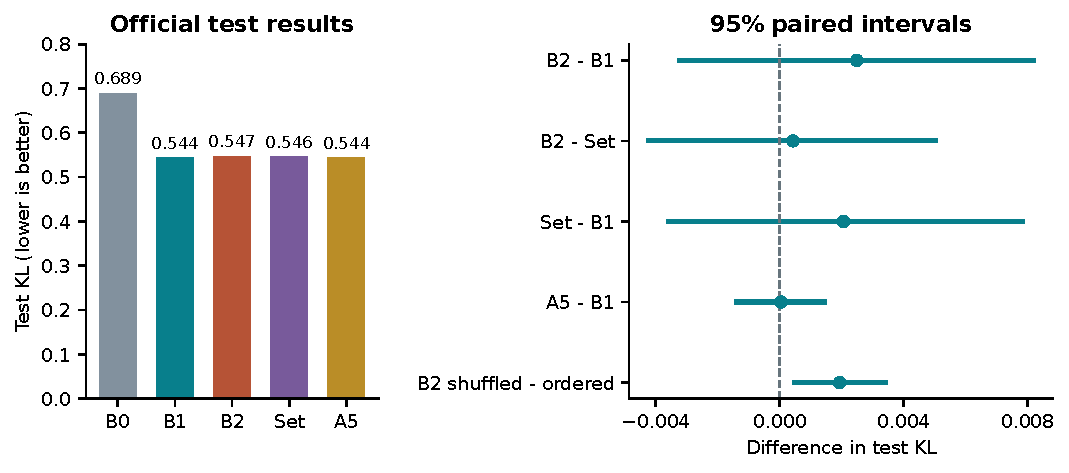
\includegraphics[width=\textwidth]{figures/results_and_uncertainty.pdf}
\caption{Left: official test KL. Right: paired KL differences for learned-model comparisons and the within-model shuffle diagnostic. Intervals show movie-cluster bootstrap uncertainty, not variation across independently trained seeds.}\label{fig:main}
\end{figure}\FloatBarrier

\subsection{Movie-cluster bootstrap}
The test set contains 1,183 distinct movies. For each of 10,000 bootstrap draws, movies were resampled with replacement and all clips belonging to each drawn movie were retained. The same resample was applied to both models in a contrast. The statistic remained the clip-weighted mean difference:
\begin{equation}
\Delta^*=\frac{\sum_m w_m\sum_{i\in m}\left[\ell_i(A)-\ell_i(B)\right]}{\sum_m w_m n_m},
\end{equation}
where $w_m$ is the multiplicity of movie $m$, $n_m$ its clip count, and $\ell_i$ the per-clip evaluation KL. Intervals are the 2.5th/97.5th percentiles; bootstrap RNG seed is 20260930, independent of the fixed training seed 42.
\tbl{bootstrap}

The B1--B0 interval is entirely negative, supporting improved KL on this benchmark. Every listed comparison between separately trained learned models includes zero. This fails to establish KL superiority; it also does not prove equivalence. These marginal intervals do not account for multiple comparisons, training-seed variability, backbone choices, or uncertainty in annotation quality. They cover KL only; small MRR/F1/cosine gains remain point estimates.

\subsection{Order sensitivity versus useful superiority}
Shuffling test frames changes B2's KL from 0.546904 to 0.548840, with maximum absolute probability change 0.128323. The paired interval for shuffled minus ordered KL is positive. B1, A5, and Set change by at most $2.4\times10^{-7}$ in predicted probability, consistent with numerical order invariance.

Thus, B2 uses frame order and performs slightly better on its original ordering than on the saved shuffled ordering. Nevertheless, B2 does not clearly beat Set or B1 in KL. The shuffle comparison is conditional on one trained model and one saved permutation per clip; it is not evidence that chronology is generally unnecessary or that B2 understands narrative causality.

\section{Failure modes, stratification, and examples}
\subsection{Class imbalance remains a major limitation}
\tbl{rare_classes}
B1 has nonzero Top-1 F1 for only fear, disapproval, amusement, and admiration. Fourteen classes are never predicted as Top-1, while three additional classes receive occasional predictions with zero true positives. Its macro Top-1 F1 over all 21 labels is 0.0979, versus official weighted F1 0.5291. These numbers use different weighting schemes and should not be directly substituted for each other.

B2's stronger weighted Top-1 score coexists with zero Top-1 predictions for 17 classes. Its Top-3 F1 is nonzero for eight classes, compared with 12 for B1 and A5. Aggregate ranking gains therefore do not establish broad improvement over the reaction taxonomy. Appendix~\ref{app:classes} reports precision, recall, F1, target support, and prediction support for every class and model.

\subsection{Stratified performance}
Bins were derived from training only. Target-entropy cut points are 1.240684, 1.490230, and 1.711419 nats; frame-count cuts are 25, 39, and 58; dominant-probability cuts are 0.346154, 0.437500, and 0.555556. Equality goes to the upper bin. The resulting test groups need not contain equal numbers of clips.
\tbl{strata}
\begin{figure}[!htbp]\centering
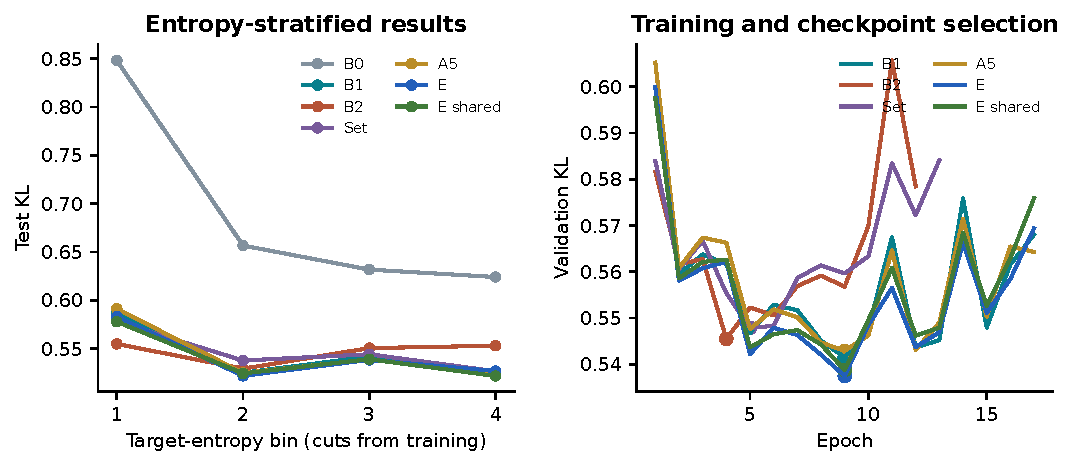
\includegraphics[width=\textwidth]{figures/diagnostics_and_training.pdf}
\caption{Left: KL across target-entropy bins defined on training. Right: validation-KL histories; dots identify the selected checkpoints. Test scores did not choose these epochs.}\label{fig:diagnostics}
\end{figure}\FloatBarrier
B1 improves over B0 in every target-entropy bin. The largest absolute gain is in the lowest-entropy group, where confident reaction targets are poorly approximated by the constant prior. B2 has the lowest KL in that bin, but its relative ordering changes in other bins. These stratified point estimates are descriptive; no separate uncertainty intervals or multiple-comparison adjustment were computed for them.

\subsection{Unseen-movie subset}
On the 84 test clips from movies absent from training, KL is 0.742025 for B0, 0.600715 for B1, 0.594232 for B2, 0.580218 for Set, and 0.597690 for A5. The small subset and absence of training-seed replication prevent reliable ranking for new-movie generalization. It is an evaluation subset of the original trained models, not a newly trained movie-disjoint benchmark.

\subsection{Twenty selected prediction examples}
Appendix~\ref{app:examples} contains five large B1 improvements over B0, five large regressions, five high-entropy clips, and five low-entropy clips. Selection is deterministic and uses distinct clips and movies across all groups. Improvements/regressions are ranked by per-clip KL difference, followed by the highest/lowest entropy among remaining clips, with sample-ID tie breaking.

These are post-hoc distribution-error illustrations, not a representative sample, a fresh evaluation set, or a basis for choosing hyperparameters. Each entry reports the clip/movie identity, frame count, entropy, B0/B1 KL, and target/B1 top-three probabilities. Complete distributions for all five models are saved in \path{research_notes/qualitative_examples.json}. Scene semantics and causal explanations have not been established by visually reviewing these clips. The examples show what the predictor gets right or wrong at the distribution level.

\section{Do the experiments actually test the hypotheses?}
\begin{description}[style=nextline]
\item[Visual prediction beyond a class prior: supported within this setup.]
B1 has visual input and a trained head; B0 is a constant fitted only from training targets. The large paired gain establishes useful visual predictive information on these official splits. Alternative sources of signal include movie appearance and pretrained semantic familiarity; causal emotional understanding is not isolated.
\item[Temporal positions improve prediction beyond matched set attention: not supported on primary test KL.]
B2 and Set are matched in capacity, initialization, loss, optimizer, and data, with positions as the intervention. Their KL difference is small and uncertain. This is counterevidence to a strong claim that this particular positional configuration improves KL, but not a rejection of all temporal modeling.
\item[Composite shape/ranking supervision improves the metric tradeoff: tentative.]
A5 changes the loss relative to B1 and has small favorable cosine/MRR/F1@3 point differences. KL is effectively unchanged at the observed precision and its interval includes zero. The two auxiliary terms are changed together, and validation KL remains the selection rule. Attribution, robustness, and optimal coefficients remain unknown.
\item[Sparse emotional peaks dominate audience reaction: untested.]
All-frame mean pooling and a positional transformer do not implement emotion-ranked Top-K selection. An order-independent mean aggregates content but does not demonstrate narrative understanding. The main peak hypothesis requires the controlled selection/fusion experiments below.
\item[VAD geometry improves prediction: untested.]
Sourced VAD coordinates were provisioned for all labels, but no VAD auxiliary or geometry-regularized model was trained. Availability and interpretability of coordinates do not establish predictive benefit. An improvement in ordinal CAD alone would not validate a three-dimensional VAD mechanism.
\end{description}

\textbf{Answer to the search-space question.} The implemented code reflects the narrow B0/B1/B2/Set/A5 hypotheses described above. The results constrain these specific configurations under one backbone, one seed, one optimization schedule, and the original splits. They cannot prove or disprove the broader architecture or loss search space. Test-set follow-ups selected after viewing these scores should be described as exploratory.

\section{Untested experiments and the next research decisions}
This section explains the remaining requested directions. It records scientific intent and appropriate controls; none of these full benchmark results is being claimed.

\subsection{Perceived emotion, peaks, and global context: C, D, E, F}
\textbf{C: perceived-emotion evidence.} A practical pretrained image-emotion model would produce a coarse distribution $a_t$. With sourced coarse-label coordinates $e_k$, frame VAD is $v_t=\sum_k a_{tk}e_k$. Compare visual features alone with visual+emotion, visual+VAD, and visual+emotion+VAD. A perceived-emotion classifier is an additional evidence source, not ground truth for induced audience reactions. A suitable pretrained model and its frozen feature cache remain to be prepared.

\textbf{D: peak selection.} The requested candidate scores are arousal, distance from a declared neutral VAD point, and confidence-weighted distance:
\begin{equation}
s_t^{(1)}=A_t,\quad s_t^{(2)}=\|v_t-v_0\|_2,\quad
s_t^{(3)}=\left(1-\frac{H(a_t)}{\log K_{\rm coarse}}\right)\|v_t-v_0\|_2.
\end{equation}
Compare $K=1,2,4,8,$ and all frames, preserving the same candidate-frame set and backbone. Equal-$K$ uniform and random selections are necessary controls: fewer frames can regularize a model independently of emotional salience. An inverted-U curve alone would not identify emotional peaks as the cause.

\textbf{E: reaction-specific attention.} For learned reaction queries $r_c$, compute $a_{ct}=\softmax_t(r_c^\top u_t/\tau)$ and pool a separate representation per reaction. A query implementation passed the three-video smoke, but full benchmark training and evaluation were not run. Compare reaction-specific queries with a shared-attention control and save frame attention. Attention weights show model behavior, not causal explanations.

\textbf{F: global-plus-peak fusion.} Concatenate global context and selected-frame representations, $h=[h_{\rm global};h_{\rm peak}]$. Compare global only, peak only, and fusion, plus an extra-capacity control. This would test complementary predictive value; it should not be described as evidence of narrative understanding merely because fusion improves a score.

\subsection{VAD supervision and geometry}
The private NRC-based asset provides sourced coordinates for all 21 reaction labels; none were silently invented. The lexicon is provisioned on the cluster rather than redistributed in this source bundle. Two planned interventions are
\begin{align}
y_{\rm VAD}&=\sum_c p_ce_c,\qquad
L=L_{\rm reaction}+\lambda_{\rm VAD}\|g(h)-y_{\rm VAD}\|_2^2,\\
L_{\rm geom}&=\sum_{c<d}\left[\cos(w_c,w_d)-\exp(-\gamma\|e_c-e_d\|_2^2)\right]^2.
\end{align}
The first adds expected-VAD regression; the second constrains classifier geometry. Matched permuted-coordinate controls are needed to distinguish emotion structure from generic auxiliary regularization. Permute only auxiliary assignments, keeping official class/CAD order unchanged. Neither intervention has been evaluated.

\subsection{Description diagnostic and optional extensions}
All clips have descriptions, so description-only and visual+description comparisons are feasible and remain important. They must be reported separately from video-only prediction. The paper reports stronger text-assisted performance \cite{paper}; this motivates a diagnostic, not an assumption that description features are available to a deployment system.

Other requested branches remain optional and unlaunched: semantic reaction prototypes (fixed, projected, or residual), training-only nearest-neighbor retrieval ($K=1,3,5,10,20$ with blend weight selected on validation), positive/negative/ambiguous hierarchical supervision, and an entropy-prediction auxiliary head. Retrieval must never use test neighbors and should include same-movie exclusion. Hierarchy and entropy experiments need controls that distinguish useful structure from added capacity or auxiliary loss alone.

\subsection{Recommended sequence}
Use B1 as the current validation-selected reference. First establish one reliable perceived-emotion feature source and implement auditable peak selection. Then run a bounded C/D/E/F batch with equal-frame-count and capacity controls, followed by the VAD and description comparisons. Preserve the fixed training recipe initially, use validation for any new selection, and record additional test-driven exploration explicitly. No new batch was launched while preparing this report.

\section{Reproduction, provenance, and cluster records}
\subsection{Exact run identities}
\begin{table}[!htbp]\centering\small
\begin{tabular}{llll}\toprule
Experiment & Job ID & Source commit & State / elapsed \\\midrule
B0 & 27382108 & \code{e91a469} & completed / 4m51s \\
Feature cache & 27382293 & \code{bbf8c1d} & completed / 1h50m35s \\
B1 & 27382294 & \code{bbf8c1d} & completed / 2m42s \\
B2 & 27382295 & \code{bbf8c1d} & completed / 2m42s \\
Set & 27382296 & \code{bbf8c1d} & completed / 2m43s \\
A5 & 27382297 & \code{bbf8c1d} & completed / 2m42s \\\bottomrule
\end{tabular}
\caption{Every listed job exited 0:0. The cache is preprocessing, not a benchmark predictor.}\label{tab:jobs}
\end{table}\FloatBarrier
The corrected immutable release is \path{releases/bbf8c1d019a4-9a6a80a3d307}. B0 used \path{releases/e91a469f51ba-b53672620486}. The analysis report and saved aggregate results were committed as \code{2a7548e}; this document describes those completed model runs and adds report diagnostics without retraining them. Full source hashes, package versions, data/model revisions, and resolved configurations accompany every run.

\subsection{Artifact map}
The Snellius project root is \path{/scratch-shared/gmago/video2reaction}. Paths below are relative to that root.
\begin{longtable}{>{\raggedright\arraybackslash}p{0.44\textwidth}>{\raggedright\arraybackslash}p{0.49\textwidth}}
\toprule Path & Contents \\\midrule\endhead
\path{code/} & Mutable synchronized working copy and cluster uv environment. \\
\path{releases/} & Frozen source snapshots used by queued and running jobs. \\
\path{data/metadata/} & Original pinned train/validation/test JSON files. \\
\path{data/key_frames} & Symlink to the existing keyframe dataset. \\
\path{data/features/siglip2-so400m/b69db8858136c6a0/} & Complete frozen features, split indices, progress/completion manifests, and checksums. \\
\path{outputs/experiments/<name>_<job>/} & Resolved config, code/environment/split provenance, metrics, checkpoints when applicable, and stdout link. \\
\path{outputs/experiments/<run>/test/} & \path{predictions.npz}, \path{metrics.json}, and \path{per_class.json}; analogous validation directory. \\
\path{logs/experiments/} and \path{logs/slurm/} & Experiment and scheduler logs. \\
\path{results/experiment_registry.json} & File-locked global registry, retaining failed attempts. \\
\path{results/collected/} & Collected summaries and paired uncertainty analysis. \\
\bottomrule
\end{longtable}
The original frames resolve to \path{/gpfs/home3/gmago/video2reaction/scratch4/workspace/sidongzhang_umass_edu-v2r/v2r_data/youtube_video/key_frames}. New work uses the organized symlink, avoiding a duplicate dataset copy. Generated predictions, checkpoints, reports, and logs are synchronized to the Mac; raw frames, raw split files, and feature tensors remain on Snellius.

\subsection{Commands to inspect and intentionally reproduce B1}
Inspect the completed runs without submitting new jobs:
\begin{verbatim}
cd /scratch-shared/gmago/video2reaction/code
source configs/clusters/snellius.env
bash scripts/status_all.sh
python3 scripts/collect_results.py --reconcile
uv run --frozen --no-sync python scripts/analyze_tier0.py \
  --outputs "$V2R_OUTPUT_DIR/experiments" \
  --output "$V2R_ROOT/results/collected/tier0_results.json"
\end{verbatim}
An intentional repeat of the original B1 configuration uses the original frozen release and the existing completed cache. A new SLURM job ID creates a separate output directory:
\begin{verbatim}
cd /scratch-shared/gmago/video2reaction/releases/\
bbf8c1d019a4-9a6a80a3d307
source configs/clusters/snellius.env
budget-overview
squeue -u "$USER"
sbatch --test-only slurm/b1_meanpool.sbatch
sbatch --output="$V2R_ROOT/logs/slurm/b1_meanpool-%j.out" \
  slurm/b1_meanpool.sbatch
\end{verbatim}
This submits a new allocation and reuses the pinned cache. The SLURM wrapper invokes \path{train.py --config configs/experiments/b1_meanpool.yaml} with a unique run name and the shared registry. \path{scripts/submit_all.sh} handles the whole first batch and duplicate-release guards; it should not be used merely to inspect results. Failed learned runs can resume from \path{last.pt} via \code{V2R\_RESUME\_FROM} when configuration/source identities match.

On the Mac, code and artifact synchronization are separate operations:
\begin{verbatim}
bash scripts/sync_cluster.sh   # code: Mac -> Snellius
bash scripts/sync_outputs.sh   # generated artifacts: Snellius -> Mac
\end{verbatim}
Neither uses destructive synchronization. Environments and raw data are excluded. Log symlinks are materialized for local readability, and \path{results/sync_receipt.json} records the transfer. CodeGraph v1.6.1 is installed on Snellius; repository indexing has not been enabled.

\subsection{Budget, storage, and access snapshot}
At 00:38 UTC on 1 October 2026, \code{budget-overview} reported account \code{gusr133332} with \textbf{87,861:20 SBU} left for dispatch and submission, and zero active/queued jobs. This is the account's remaining allocation, not the cost of this batch alone. SURF's tool combines registered budget with recent SLURM usage \cite{surf}.

Home quota usage was 40.4098\% of 200 GiB: about 80.82 GiB used and 119.18 GiB available under the quota; 699,411 of 1,000,000 nominal inodes were used. Scratch usage was 0.1124\% of an 8 TiB quota, leaving approximately 7.991 TiB; inode usage was 1.2616\% of 3,000,000. The feature directory occupied about 2.1 GiB and experiment outputs about 70 MiB by \code{du}. Quota percentages and \code{du} are different measurements and are reported at their observed precision. Scratch is temporary storage.

Snellius GPU A100/H100/MIG and relevant build/staging products were verified under the account; only Snellius was used for these experiments. UvA access was inspected earlier but no project job was submitted there. New submissions still require a current account/partition check and \code{sbatch --test-only}. These report-generation steps did not change model weights or launch a new training batch.

\section{Conclusions}
\textbf{Current working model.} B1 is the simplest trained reference and the lowest-validation-KL configuration. Its visual improvement over the prior is substantial and supported by paired test-sample uncertainty analysis.

\textbf{Supported, tentative, and untested claims.} Visual features add predictive information under the official split. B2 uses order, but a clear advantage over a matched set model was not demonstrated. A5 offers small descriptive ranking/cosine gains. The experiments do not establish a general winner between learned models, broad rare-class competence, new-movie generalization, or dominance over published systems using different modalities and training regimes.

\textbf{Peaks, global context, and VAD.} The central peak-versus-context question remains unanswered because the required peak and fusion interventions were not run. Mean pooling is evidence for useful aggregate visual content, not proof of narrative reasoning. VAD coordinates are available, but there is no trained VAD result from which to infer predictive benefit. The next controlled experiments must supply this missing evidence rather than reinterpret Tier 0 as a test of hypotheses it did not implement.

\clearpage
\begin{thebibliography}{9}
\bibitem{paper} T. Nguyen, S. Zhang, S. Shankar, G. Jagatap, D. Chandran, A. Fanelli, and M. Fiterau.
\emph{Video2Reaction: Mapping Video to Audience Reaction Distribution in the Wild}. arXiv:2607.06875v1, 2026.
\url{https://arxiv.org/abs/2607.06875v1}.
\bibitem{dataset} Information Fusion Lab. \emph{Video2Reaction dataset and metadata}. Pinned revision \nolinkurl{578d1423f89f1a7b52471b01e78770e08f0a226c}.
\url{https://huggingface.co/datasets/infofusionlab/Video2Reaction}.
\bibitem{siglip} Google. \emph{SigLIP2 SO400M patch14/384 model}. Pinned revision \nolinkurl{e8e487298228002f3d8a82e0cd5c8ea9c567f57f}.
\url{https://huggingface.co/google/siglip2-so400m-patch14-384}.
\bibitem{results} Video2Reaction research branch. \emph{Completed Tier 0 results, diagnostics, and paired KL analysis}. Commit \code{2a7548e}, 30 September 2026.
\url{https://github.com/gowreesh-mago/video2reaction/blob/2a7548e/research_notes/tier0_results.json}.
\bibitem{code} Video2Reaction research branch. \emph{Corrected training and feature-extraction source}. Commit \code{bbf8c1d}; B0 source \code{e91a469}.
\url{https://github.com/gowreesh-mago/video2reaction/tree/bbf8c1d}.
\bibitem{surf} SURF. \emph{Getting account and budget information}. Accessed 1 October 2026.
\url{https://servicedesk.surf.nl/wiki/spaces/WIKI/pages/300974118/Getting+account+and+budget+information}.
\end{thebibliography}

\appendix
\clearpage
\section{Class taxonomy and target imbalance}\label{app:taxonomy}
The row order below is the fixed order used by predictions and ordinal CAD. It is not alphabetical. The three most frequent reactions dominate the probability mass, while several labels never appear as metadata-dominant reactions in training.
\tbl{taxonomy}

\clearpage
\section{Per-class results for every completed model}\label{app:classes}
The tables below use saved official test top-k sets. All scores are proportions. $P_k$, $R_k$, and $F_k$ are class precision, recall, and F1; $S_k$ counts target top-k membership, while $N_k$ counts predicted membership. Each clip contributes exactly $k$ memberships, including the official tie/zero-probability conventions. Undefined scores are zero. A zero with no target support is not evidence that a model learned or failed to learn that class.
\tbl{classes_b0_prior}
\tbl{classes_b1_meanpool}
\tbl{classes_b2_temporal}
\tbl{classes_b2_set_control}
\tbl{classes_a5_distribution}

\clearpage
\section{Twenty prediction examples}\label{app:examples}
These are selected distribution diagnostics from completed test predictions. They were not used to train or select a checkpoint. All 20 clips and movie IDs are distinct. Hyperlinks use the saved YouTube IDs; current playback availability was not checked. Only the top-three probabilities are displayed, so displayed mass generally sums to less than one. The JSON companion contains all 21 target probabilities and all five predicted distributions.

\subsection{Five large improvements over the class prior}
These clips have the largest retained positive reductions $\KL(B0)-\KL(B1)$, enforcing movie diversity. They demonstrate that the visual head can recover reactions poorly represented by a global prior, but selected extremes do not measure typical gain.
\par\noindent\begin{minipage}{\textwidth}\small
\textbf{Q01}\quad\href{https://www.youtube.com/watch?v=mExTnHwAcYY}{\texttt{mExTnHwAcYY}}\quad IMDb: \texttt{tt0120686}\par
\textit{Stepmom}\par
Frames: 18; target entropy: 1.109 nats; KL(B0): 3.127; KL(B1): 0.831.\par
Target top 3: grief 0.543, sadness 0.314, admiration 0.086.\par
B1 top 3: admiration 0.339, sadness 0.165, grief 0.158.\par
\end{minipage}\par\medskip
\par\noindent\begin{minipage}{\textwidth}\small
\textbf{Q02}\quad\href{https://www.youtube.com/watch?v=KJtfL83FLj8}{\texttt{KJtfL83FLj8}}\quad IMDb: \texttt{tt3607812}\par
\textit{The Sheik}\par
Frames: 31; target entropy: 1.226 nats; KL(B0): 2.851; KL(B1): 1.090.\par
Target top 3: sadness 0.429, grief 0.393, caring 0.071.\par
B1 top 3: disapproval 0.244, admiration 0.184, sadness 0.139.\par
\end{minipage}\par\medskip
\par\noindent\begin{minipage}{\textwidth}\small
\textbf{Q03}\quad\href{https://www.youtube.com/watch?v=aY6ZwMZqaBk}{\texttt{aY6ZwMZqaBk}}\quad IMDb: \texttt{tt1398426}\par
\textit{Straight Outta Compton}\par
Frames: 20; target entropy: 1.137 nats; KL(B0): 2.774; KL(B1): 1.206.\par
Target top 3: sadness 0.533, grief 0.267, admiration 0.133.\par
B1 top 3: admiration 0.431, disapproval 0.140, sadness 0.115.\par
\end{minipage}\par\medskip
\par\noindent\begin{minipage}{\textwidth}\small
\textbf{Q04}\quad\href{https://www.youtube.com/watch?v=hn09SKCZgtI}{\texttt{hn09SKCZgtI}}\quad IMDb: \texttt{tt0098384}\par
\textit{Steel Magnolias}\par
Frames: 15; target entropy: 1.286 nats; KL(B0): 2.430; KL(B1): 1.016.\par
Target top 3: grief 0.564, admiration 0.179, disapproval 0.103.\par
B1 top 3: admiration 0.300, disapproval 0.193, sadness 0.114.\par
\end{minipage}\par\medskip
\par\noindent\begin{minipage}{\textwidth}\small
\textbf{Q05}\quad\href{https://www.youtube.com/watch?v=jYbI8iVYCpc}{\texttt{jYbI8iVYCpc}}\quad IMDb: \texttt{tt4786282}\par
\textit{Lights Out}\par
Frames: 39; target entropy: 0.951 nats; KL(B0): 2.034; KL(B1): 0.629.\par
Target top 3: fear 0.632, confusion 0.263, disapproval 0.053.\par
B1 top 3: fear 0.379, disapproval 0.120, surprise 0.086.\par
\end{minipage}\par\medskip

\clearpage
\subsection{Five large regressions relative to the prior}
These have the largest retained increases in KL from using B1. They are clear failures relative to the simple baseline. The displayed probabilities reveal the mismatch without assigning an unverified scene-level cause.
\par\noindent\begin{minipage}{\textwidth}\small
\textbf{Q06}\quad\href{https://www.youtube.com/watch?v=pDj1GM3RRWs}{\texttt{pDj1GM3RRWs}}\quad IMDb: \texttt{tt0389860}\par
\textit{Click}\par
Frames: 44; target entropy: 1.516 nats; KL(B0): 2.435; KL(B1): 3.586.\par
Target top 3: grief 0.371, sadness 0.371, surprise 0.086.\par
B1 top 3: amusement 0.285, disapproval 0.240, admiration 0.227.\par
\end{minipage}\par\medskip
\par\noindent\begin{minipage}{\textwidth}\small
\textbf{Q07}\quad\href{https://www.youtube.com/watch?v=I0YUjv1u-Gw}{\texttt{I0YUjv1u-Gw}}\quad IMDb: \texttt{tt0119715}\par
\textit{Mousehunt}\par
Frames: 15; target entropy: 1.446 nats; KL(B0): 1.064; KL(B1): 2.107.\par
Target top 3: admiration 0.500, joy 0.150, approval 0.150.\par
B1 top 3: amusement 0.667, disapproval 0.078, admiration 0.074.\par
\end{minipage}\par\medskip
\par\noindent\begin{minipage}{\textwidth}\small
\textbf{Q08}\quad\href{https://www.youtube.com/watch?v=ARTwLLhQZHw}{\texttt{ARTwLLhQZHw}}\quad IMDb: \texttt{tt2557490}\par
\textit{A Million Ways to Die in the West}\par
Frames: 24; target entropy: 0.349 nats; KL(B0): 1.223; KL(B1): 2.039.\par
Target top 3: amusement 0.889, admiration 0.111, joy 0.000.\par
B1 top 3: admiration 0.620, joy 0.153, amusement 0.072.\par
\end{minipage}\par\medskip
\par\noindent\begin{minipage}{\textwidth}\small
\textbf{Q09}\quad\href{https://www.youtube.com/watch?v=1pzV9GoSuys}{\texttt{1pzV9GoSuys}}\quad IMDb: \texttt{tt1210166}\par
\textit{Moneyball}\par
Frames: 15; target entropy: 1.615 nats; KL(B0): 0.538; KL(B1): 1.298.\par
Target top 3: disapproval 0.484, approval 0.129, admiration 0.129.\par
B1 top 3: amusement 0.734, admiration 0.098, disapproval 0.083.\par
\end{minipage}\par\medskip
\par\noindent\begin{minipage}{\textwidth}\small
\textbf{Q10}\quad\href{https://www.youtube.com/watch?v=k3oMPqUTxCE}{\texttt{k3oMPqUTxCE}}\quad IMDb: \texttt{tt0061512}\par
\textit{Cool Hand Luke}\par
Frames: 59; target entropy: 1.447 nats; KL(B0): 0.423; KL(B1): 1.176.\par
Target top 3: amusement 0.471, admiration 0.235, disapproval 0.118.\par
B1 top 3: disapproval 0.241, disgust 0.194, admiration 0.187.\par
\end{minipage}\par\medskip

\clearpage
\subsection{Five high-entropy examples}
These are the highest-entropy remaining clips after the improvement/failure examples and movie-diversity exclusions. Their targets are more dispersed across reactions; a dominant-label score alone omits much of that structure.
\par\noindent\begin{minipage}{\textwidth}\small
\textbf{Q11}\quad\href{https://www.youtube.com/watch?v=FMbSH8g9vsU}{\texttt{FMbSH8g9vsU}}\quad IMDb: \texttt{tt0837563}\par
\textit{Pet Sematary}\par
Frames: 30; target entropy: 2.401 nats; KL(B0): 0.644; KL(B1): 0.510.\par
Target top 3: admiration 0.143, confusion 0.143, joy 0.095.\par
B1 top 3: admiration 0.190, disapproval 0.182, confusion 0.129.\par
\end{minipage}\par\medskip
\par\noindent\begin{minipage}{\textwidth}\small
\textbf{Q12}\quad\href{https://www.youtube.com/watch?v=okdTt3VfJ6s}{\texttt{okdTt3VfJ6s}}\quad IMDb: \texttt{tt3713166}\par
\textit{Unfriended}\par
Frames: 15; target entropy: 2.341 nats; KL(B0): 0.494; KL(B1): 0.182.\par
Target top 3: disapproval 0.226, disgust 0.161, admiration 0.161.\par
B1 top 3: disapproval 0.286, disgust 0.102, confusion 0.101.\par
\end{minipage}\par\medskip
\par\noindent\begin{minipage}{\textwidth}\small
\textbf{Q13}\quad\href{https://www.youtube.com/watch?v=dVCki9kwF_4}{\texttt{dVCki9kwF\_4}}\quad IMDb: \texttt{tt1060277}\par
\textit{Cloverfield}\par
Frames: 39; target entropy: 2.229 nats; KL(B0): 0.417; KL(B1): 0.166.\par
Target top 3: fear 0.250, admiration 0.196, disapproval 0.152.\par
B1 top 3: disapproval 0.254, admiration 0.204, fear 0.136.\par
\end{minipage}\par\medskip
\par\noindent\begin{minipage}{\textwidth}\small
\textbf{Q14}\quad\href{https://www.youtube.com/watch?v=BcW6m0Rg1-8}{\texttt{BcW6m0Rg1-8}}\quad IMDb: \texttt{tt0430105}\par
\textit{Four Brothers}\par
Frames: 38; target entropy: 2.206 nats; KL(B0): 0.546; KL(B1): 1.034.\par
Target top 3: disapproval 0.360, surprise 0.080, fear 0.080.\par
B1 top 3: amusement 0.490, disapproval 0.187, admiration 0.124.\par
\end{minipage}\par\medskip
\par\noindent\begin{minipage}{\textwidth}\small
\textbf{Q15}\quad\href{https://www.youtube.com/watch?v=SfL4U_bOGvc}{\texttt{SfL4U\_bOGvc}}\quad IMDb: \texttt{tt0380510}\par
\textit{The Lovely Bones}\par
Frames: 44; target entropy: 2.203 nats; KL(B0): 0.446; KL(B1): 0.476.\par
Target top 3: admiration 0.297, fear 0.162, disapproval 0.135.\par
B1 top 3: admiration 0.283, disapproval 0.234, amusement 0.093.\par
\end{minipage}\par\medskip

\clearpage
\subsection{Five low-entropy examples}
These are the lowest-entropy remaining clips under the same exclusions. Their concentrated targets make diffuse or confidently incorrect predictions especially visible. High certainty in an aggregated annotation is not a direct measure of annotation correctness.
\par\noindent\begin{minipage}{\textwidth}\small
\textbf{Q16}\quad\href{https://www.youtube.com/watch?v=4jsUIgchHXU}{\texttt{4jsUIgchHXU}}\quad IMDb: \texttt{tt0054698}\par
\textit{Breakfast at Tiffany's}\par
Frames: 15; target entropy: -0.000 nats; KL(B0): 1.302; KL(B1): 0.968.\par
Target top 3: admiration 1.000, joy 0.000, amusement 0.000.\par
B1 top 3: admiration 0.380, amusement 0.259, disapproval 0.122.\par
\end{minipage}\par\medskip
\par\noindent\begin{minipage}{\textwidth}\small
\textbf{Q17}\quad\href{https://www.youtube.com/watch?v=Sj_A7OZz8TI}{\texttt{Sj\_A7OZz8TI}}\quad IMDb: \texttt{tt0129387}\par
\textit{There's Something About Mary}\par
Frames: 23; target entropy: -0.000 nats; KL(B0): 1.606; KL(B1): 0.364.\par
Target top 3: amusement 1.000, joy 0.000, admiration 0.000.\par
B1 top 3: amusement 0.695, disapproval 0.077, admiration 0.059.\par
\end{minipage}\par\medskip
\par\noindent\begin{minipage}{\textwidth}\small
\textbf{Q18}\quad\href{https://www.youtube.com/watch?v=7EcK-LuhzAA}{\texttt{7EcK-LuhzAA}}\quad IMDb: \texttt{tt1114740}\par
\textit{Paul Blart: Mall Cop}\par
Frames: 60; target entropy: 0.238 nats; KL(B0): 1.407; KL(B1): 0.375.\par
Target top 3: amusement 0.949, disapproval 0.026, disappointment 0.026.\par
B1 top 3: amusement 0.606, admiration 0.121, disapproval 0.103.\par
\end{minipage}\par\medskip
\par\noindent\begin{minipage}{\textwidth}\small
\textbf{Q19}\quad\href{https://www.youtube.com/watch?v=_YYmfM2TfUA}{\texttt{\_YYmfM2TfUA}}\quad IMDb: \texttt{tt0075148}\par
\textit{Rocky}\par
Frames: 22; target entropy: 0.264 nats; KL(B0): 1.131; KL(B1): 0.691.\par
Target top 3: admiration 0.941, excitement 0.029, amusement 0.029.\par
B1 top 3: admiration 0.429, disapproval 0.180, amusement 0.179.\par
\end{minipage}\par\medskip
\par\noindent\begin{minipage}{\textwidth}\small
\textbf{Q20}\quad\href{https://www.youtube.com/watch?v=W7xrlkbp0Hs}{\texttt{W7xrlkbp0Hs}}\quad IMDb: \texttt{tt0218839}\par
\textit{Best in Show}\par
Frames: 15; target entropy: 0.271 nats; KL(B0): 1.475; KL(B1): 0.871.\par
Target top 3: amusement 0.923, disgust 0.077, joy 0.000.\par
B1 top 3: amusement 0.375, disapproval 0.236, admiration 0.142.\par
\end{minipage}\par\medskip


\clearpage
\section{Data and source identities}
The original metadata files have the following SHA-256 identities:
\begin{itemize}
\item Train: \nolinkurl{22f73252c6886449cd91d35989fa15b2b19e0067abcf2dfab624fcadff0fccd0}.
\item Validation: \nolinkurl{c78e6ed759d449041d8c0ff468098d71b829cb5a4d7e457d4710b2c2386acc83}.
\item Test: \nolinkurl{58558f5694f3d038ac4c6af22e5a0f2b388b43236de9ab4ba74300adb0cc672d}.
\end{itemize}
The source aggregate used for this document, \path{research_notes/tier0_results.json}, has SHA-256
\nolinkurl{a06f2eeae6ad1fe03ffbac8b2ae93b62b47696669badfece3c8513b9d8f0408a}.
The document's \path{report_manifest.json} identifies its source data and checks. Generated tables are populated from the saved cluster metrics and per-class files, rather than manually transcribed values. The two scientific figures show the same saved scores, intervals, and training histories.

The source bundle contains this main \LaTeX{} file, generated table fragments, vector figures, result JSON, example JSON, and build instructions. Compile with \code{latexmk -pdf video2reaction\_report.tex}. Regenerating the tables and figures from the repository uses \path{scripts/build_report_assets.py}; this only reads generated run artifacts and does not train models or read the full dataset.
\end{document}
